%% document class file for the preparation of a paper
%% for the International Conference ICCAS 2026
%% global option 'fleqn' ensures equations flush left.
%% set '10pt' and 'twocolumn' options.

\documentclass[10pt,twocolumn]{ICCAS}

\usepackage{amsmath,amssymb,amsfonts}
\usepackage{graphicx}
\usepackage{float}
\usepackage{booktabs}
\usepackage{diagbox}

\makeatletter
\long\def\@makecaption#1#2#3{
    \vskip 0pt
    \noindent\hbox to\hsize{\hfil\parbox{0.96\hsize}{\centering #1~ #2}\hfil}
}
\makeatother

\setlength{\textfloatsep}{14pt plus 2pt minus 2pt}
\setlength{\dbltextfloatsep}{8pt plus 2pt minus 2pt}
\makeatletter
\def\section{\@startsection {section}{1}{\z@}{4.5ex plus 0.5ex
     minus .2ex}{1.2ex}{\center\fontsize{11pt}{11pt}\rm\bf\MakeUppercaseBlue}}
\def\subsection{\@startsection{subsection}{2}{\z@}{1.2ex
     }{0.4ex}{\noindent\rm\bf\textcolor[RGB]{0,112,192}}}
\makeatother

\begin{document}

\title{Bridging the Sim-to-Real Gap in Quadrupedal Visual Navigation via 3D Gaussian Splatting}

\author{Minseok Lee${}^{1}$, Seongyu Han${}^{1}$, Heejae Moon${}^{1}$, and Sung Soo Hwang${}^{1*}$ }

\affils{ ${}^{1}$School of Artificial Intelligence, Computer and Electrical Engineering, \\
Handong Global University, Pohang 37554, Republic of Korea \\
(\{glen, tjsrb439, 22000249\}@handong.ac.kr, sshwang@handong.edu) {\small${}^{*}$ Corresponding author}}

\abstract{
    Deploying visual navigation on physical quadrupedal robots is challenging due to the visual sim-to-real gap and locomotion-induced camera jitter. This jitter degrades feature tracking and depth consistency. This paper presents a pipeline that bridges these perceptual and dynamic gaps to enable virtual parameter optimization. In the simulation stage, we reconstruct a 3D Gaussian Splatting (3DGS) digital twin of a campus corridor and use a reinforcement learning (RL) locomotion policy to generate camera bobbing noise. Under these simulated visual and dynamic disturbances, the parameters of the RTAB-Map visual SLAM and Nav2 stacks are optimized. For deployment, the RL policy is bypassed, and velocity commands are routed directly to the physical robot's built-in Sport API via a ROS 2 bridge. Real-world experiments demonstrate that parameters optimized under simulated jitter transfer directly to the physical platform, supporting visual mapping and qualitative obstacle-aware replanning without manual recalibration.
}

\keywords{
    Quadrupedal Locomotion, Visual SLAM, Sim-to-Real Pipeline, 3D Gaussian Splatting, Ego-motion Jitter, Virtual Sandbox.
}

\maketitle

\begin{figure*}[t]
\begin{center}
\vspace{-2mm}
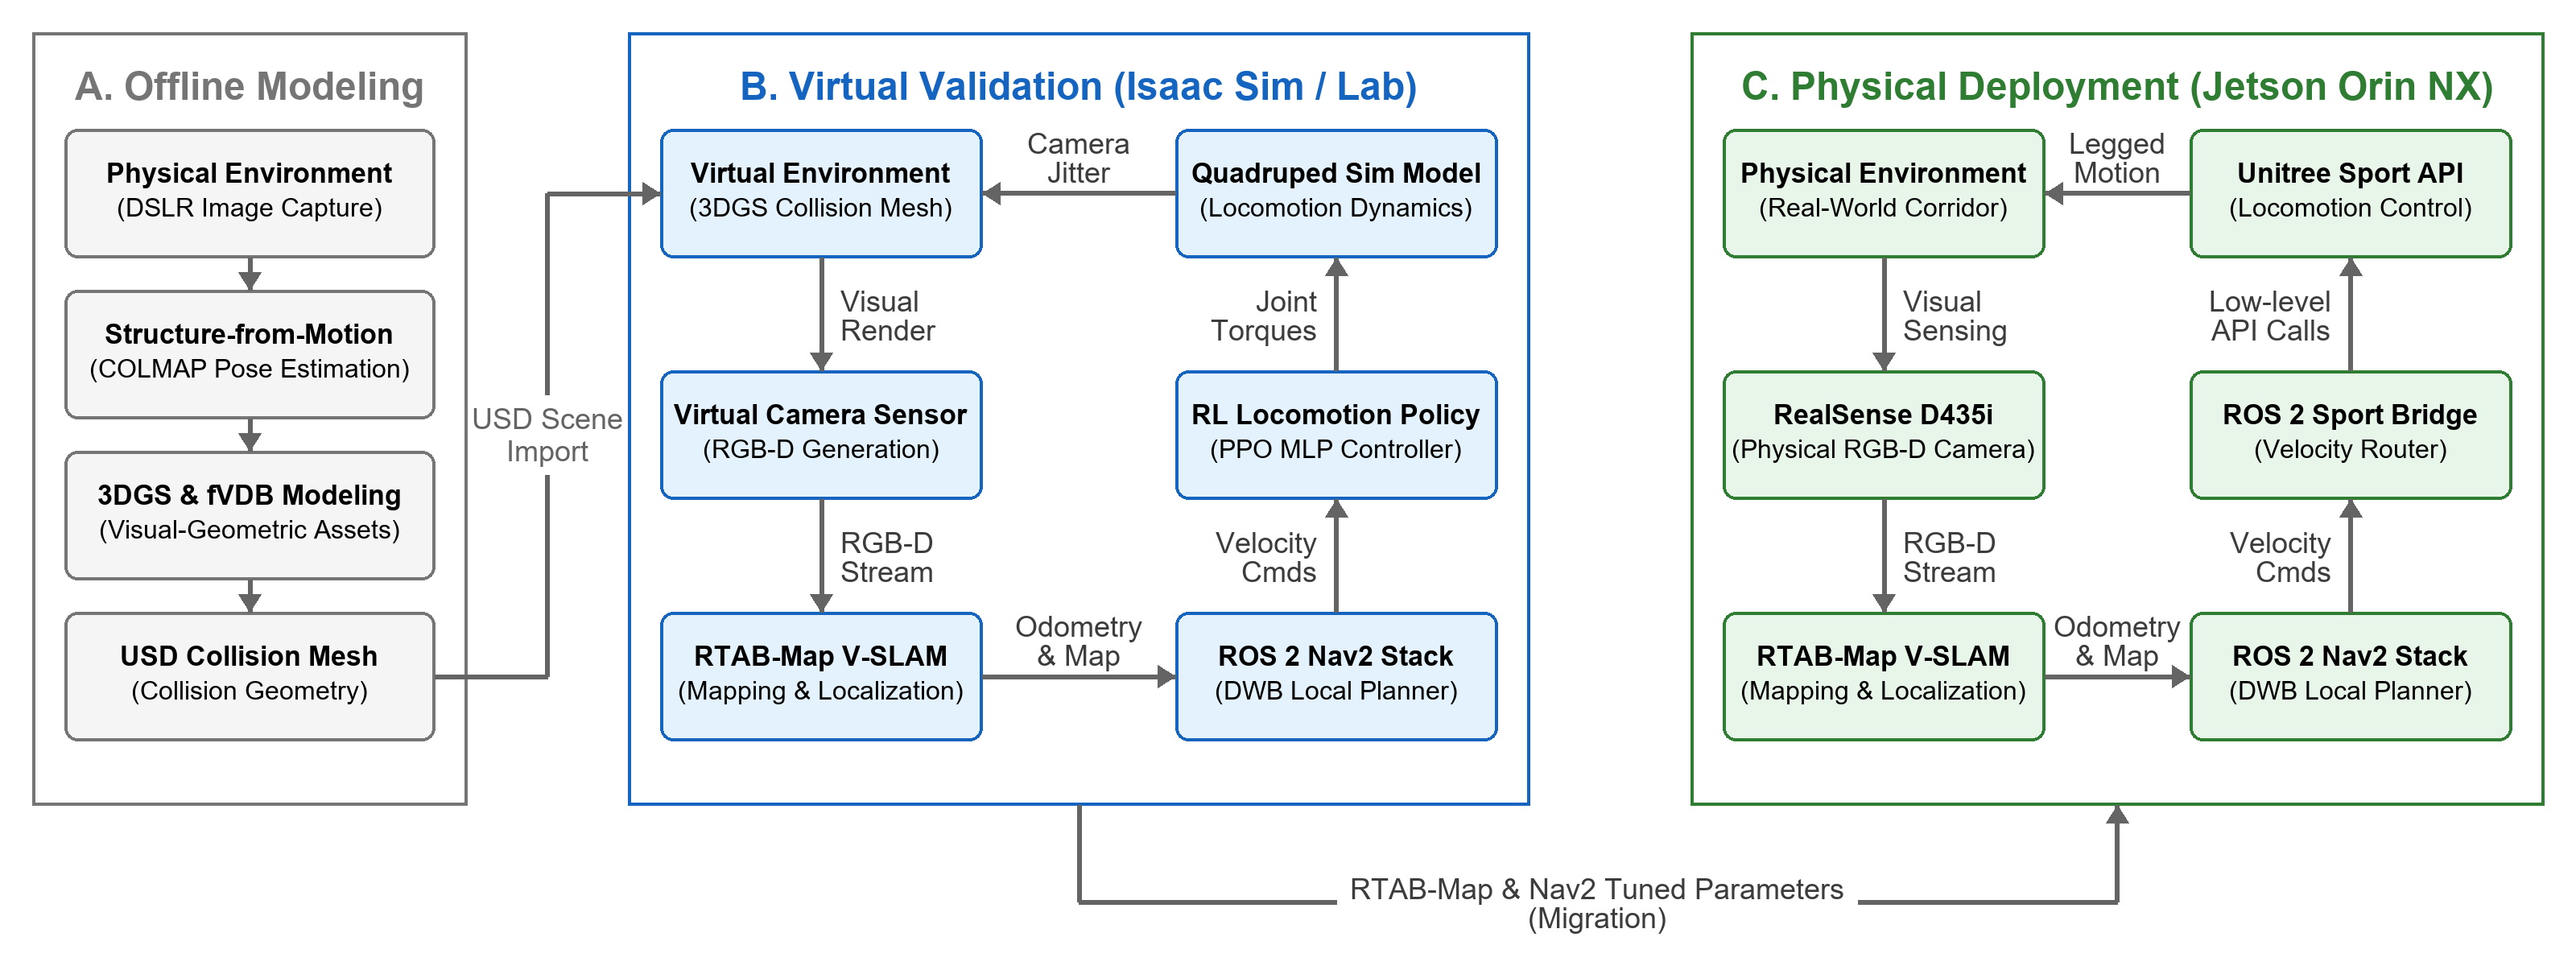
\includegraphics[width=\textwidth]{figures/fig_system_overview}
\vspace{1mm}
\caption{\label{fig_system_overview}Overall architecture of the proposed Sim-to-Real quadrupedal navigation framework. (a) In the virtual validation stage, we reconstruct a 3DGS environment and train an RL locomotion policy to emulate camera bobbing noise. (b) In the physical deployment stage, the RL policy is bypassed, and commands are sent to the Unitree Sport API via a ROS 2 bridge to reduce computational load on the Jetson Orin NX.}
\vspace{-3.5mm}
\end{center}
\end{figure*}

%-----------------------------------------------------------------------

\section{Introduction}
Autonomous quadrupedal robots offer superior mobility over wheeled systems on challenging terrains. Achieving indoor autonomy requires integrating legged locomotion with simultaneous localization and mapping (SLAM). While indoor navigation has conventionally relied on LiDAR sensors, they are heavy and power-intensive. Visual navigation using a single RGB-D camera is a lightweight, cost-effective alternative.

However, legged visual navigation introduces two primary sim-to-real challenges. First is the \textit{perceptual gap}: standard simulators lack photorealistic textures and depth fidelity, causing visual SLAM to fail in the real world due to feature matching errors. Second is the \textit{dynamic gap}: legged locomotion generates camera bobbing that causes motion blur and false obstacle detection (phantom obstacles). Furthermore, tuning parameters directly on physical hardware is limited by battery capacity and collision risks.

To address these challenges, we present a pipeline that decouples simulation-based parameter verification from physical deployment. Using a single front-facing RGB-D camera (Intel RealSense D435i) and offline 3DGS reconstruction from DSLR images, we align virtual and physical camera properties to reduce sensor discrepancy. In simulation, we reconstruct a digital twin of an indoor corridor. Since the robot's low-level controller is proprietary, we train an RL locomotion policy in Isaac Lab to emulate physical gait oscillations, generating representative camera noise. In this virtual environment, we optimize the RTAB-Map and Nav2 parameters. During physical deployment, the computationally intensive RL policy is bypassed, and velocity commands are routed directly to the manufacturer's Sport API via a ROS 2 bridge, conserving edge computing resources for SLAM and path planning.

In summary, this work establishes a photorealistic validation environment by integrating DSLR-based 3DGS and \textit{fVDB} reconstruction into a physics simulator while aligning the virtual camera with the physical sensor. It further uses an RL locomotion policy to emulate legged walking dynamics and verifies on a physical Unitree Go2 that parameters optimized under simulated disturbances can transfer without recalibration.

The remainder of this paper is organized as follows: Section 2 reviews related work. Section 3 describes the system architecture, locomotion learning, and environment construction. Section 4 details the navigation configuration, simulated validation, and real-world deployment results. Finally, Section 5 concludes this paper.

\section{Related Work}
Reinforcement learning (RL) has advanced legged control \cite{ref1}. Prior studies have transferred quadrupedal policies through actuator modeling, domain randomization, and massively parallel training \cite{ref6,ref7}. However, most legged RL research focuses on gait stability, leaving visual navigation integration and sensor noise characteristics unaddressed.

Mobile robot navigation has traditionally relied on LiDAR sensors, which are heavy and power-intensive for payload-constrained quadruped robots. Visual SLAM (VSLAM) using RGB-D cameras offers a lightweight alternative, with ORB-SLAM2 \cite{ref8} and RTAB-Map \cite{ref2} providing practical foundations for camera-based mapping. For path planning and obstacle avoidance, the ROS 2 Navigation (Nav2) framework \cite{ref3} is widely used.

Photorealistic reconstruction methods provide another route to reducing the perceptual sim-to-real gap. Structure-from-Motion pipelines such as COLMAP \cite{ref9} estimate camera poses, while 3DGS \cite{ref4} enables real-time photorealistic rendering from reconstructed scenes. Recent Gaussian-based SLAM systems such as SplaTAM \cite{ref10} also show the relevance of explicit Gaussian scene representations for dense RGB-D tracking and mapping. Although frameworks like \mbox{VR-Robo} \cite{ref5} use 3DGS to build digital twins, they often rely on heterogeneous sensors, introducing device-level discrepancies in lens distortion and field-of-view (FOV). In contrast, our pipeline configures the virtual camera to match the physical D435i sensor, minimizing visual discrepancies.

\section{System and Locomotion Control}
\subsection{System Architecture}

Our framework integrates RTAB-Map, Nav2, and a dual-stage locomotion control architecture. In simulation, a DRL policy—trained via PPO in Isaac Lab (v2.3.2) on Isaac Sim (v5.1.0)—generates camera bobbing noise. High-level velocity commands ($\mathbf{v}_{cmd} = [v_x, v_y, \omega_z]^T$) from the Nav2 local planner are mapped directly to the policy's action space. During real-world deployment, the DRL policy is bypassed, and velocity commands are routed directly to the Unitree Sport API via a ROS 2 bridge. This architecture reduces the computational load on the Jetson Orin NX. The system architecture is shown in Fig.~\ref{fig_system_overview}.

\subsection{Locomotion Learning in Isaac Sim}

To simulate camera bobbing noise, we train an RL policy in NVIDIA Isaac Lab (v2.3.2) on the Isaac Sim (v5.1.0) physics engine. The policy functions to generate walking-induced oscillations. We construct a training environment with mixed terrains (uneven ground, ramps, step obstacles) using the Procedural Terrain Generator and scale terrain difficulty via curriculum learning. To enhance policy robustness, we apply the following domain randomizations:
\begin{itemize}
    \item Torso mass randomization: $\Delta m \in [-1.0, +3.0]$~kg.
    \item Ground friction coefficient: $\mu \in [0.6, 0.8]$.
    \item External disturbances: impulse force perturbations applied to the robot's center of mass (CoM).
\end{itemize}
The physics step is 200~Hz, and the policy executes at 50~Hz. Training uses the PPO implementation in the PyTorch-based \textit{skrl} library. Both actor and critic networks are MLPs with hidden layers of $[512, 256, 128]$ and ELU activation functions. The learning rate is $1.0 \times 10^{-3}$, regulated by a KL-divergence scheduler. The discount factor is $\gamma=0.99$, and the GAE parameter is $\lambda=0.95$.

The reward function tracks velocity references while maintaining legged stability. The total reward $R$ is:
\begin{equation}
R = w_{lin} R_{lin} + w_{ang} R_{ang} + w_{air} R_{air} - \sum_{i} w_{p,i} P_{i} \label{eq_reward}
\end{equation}
where:
\begin{itemize}
    \item $R_{lin} = \exp(-\|\mathbf{v}_{xy}^* - \mathbf{v}_{xy}\|_2^2 / \sigma_{lin}^2)$ is the linear velocity tracking reward ($\mathbf{v}_{xy}^*$ and $\mathbf{v}_{xy}$ are target and actual velocities, $w_{lin} = 1.5, \sigma_{lin} = 0.25$).
    \item $R_{ang} = \exp(-(\omega_{z}^* - \omega_{z})^2 / \sigma_{ang}^2)$ is the angular velocity tracking reward ($\omega_{z}^*$ and $\omega_{z}$ are target and actual yaw rates, $w_{ang} = 0.75, \sigma_{ang} = 0.25$).
    \item $R_{air}$ is the foot clearance air-time reward ($w_{air} = 0.25$).
    \item $P_i$ represents penalty terms for base vertical velocity, roll/pitch oscillations, joint limits, excessive torque, joint acceleration, and unintended contact ($w_{p,i}$ are penalty weights).
\end{itemize}

\subsection{3DGS Environment Construction \& Agent Deployment}
We capture corridor images using a DSLR camera to avoid compression artifacts. These images serve as input to COLMAP \cite{ref9} for Structure-from-Motion (SfM) to resolve camera poses. Then, a 3DGS \cite{ref4} model is optimized and exported as a USDZ asset for visual rendering, alongside a PLY mesh for coarse geometry. For physical collision modeling, we integrate the scene with NVIDIA's sparse volumetric framework, \textit{fVDB}. The resulting digital twin, combining visual photorealism and physical collision boundaries, is shown in Fig.~\ref{fig_3dgs_mesh}. We utilize the high-fidelity 3DGS model for camera rendering (Fig.~\ref{fig_3dgs_mesh}, right) and the corresponding fVDB sparse volumetric mesh for collision detection and robot-environment contact simulation (Fig.~\ref{fig_3dgs_mesh}, left).

\begin{figure}[!t]
\begin{center}
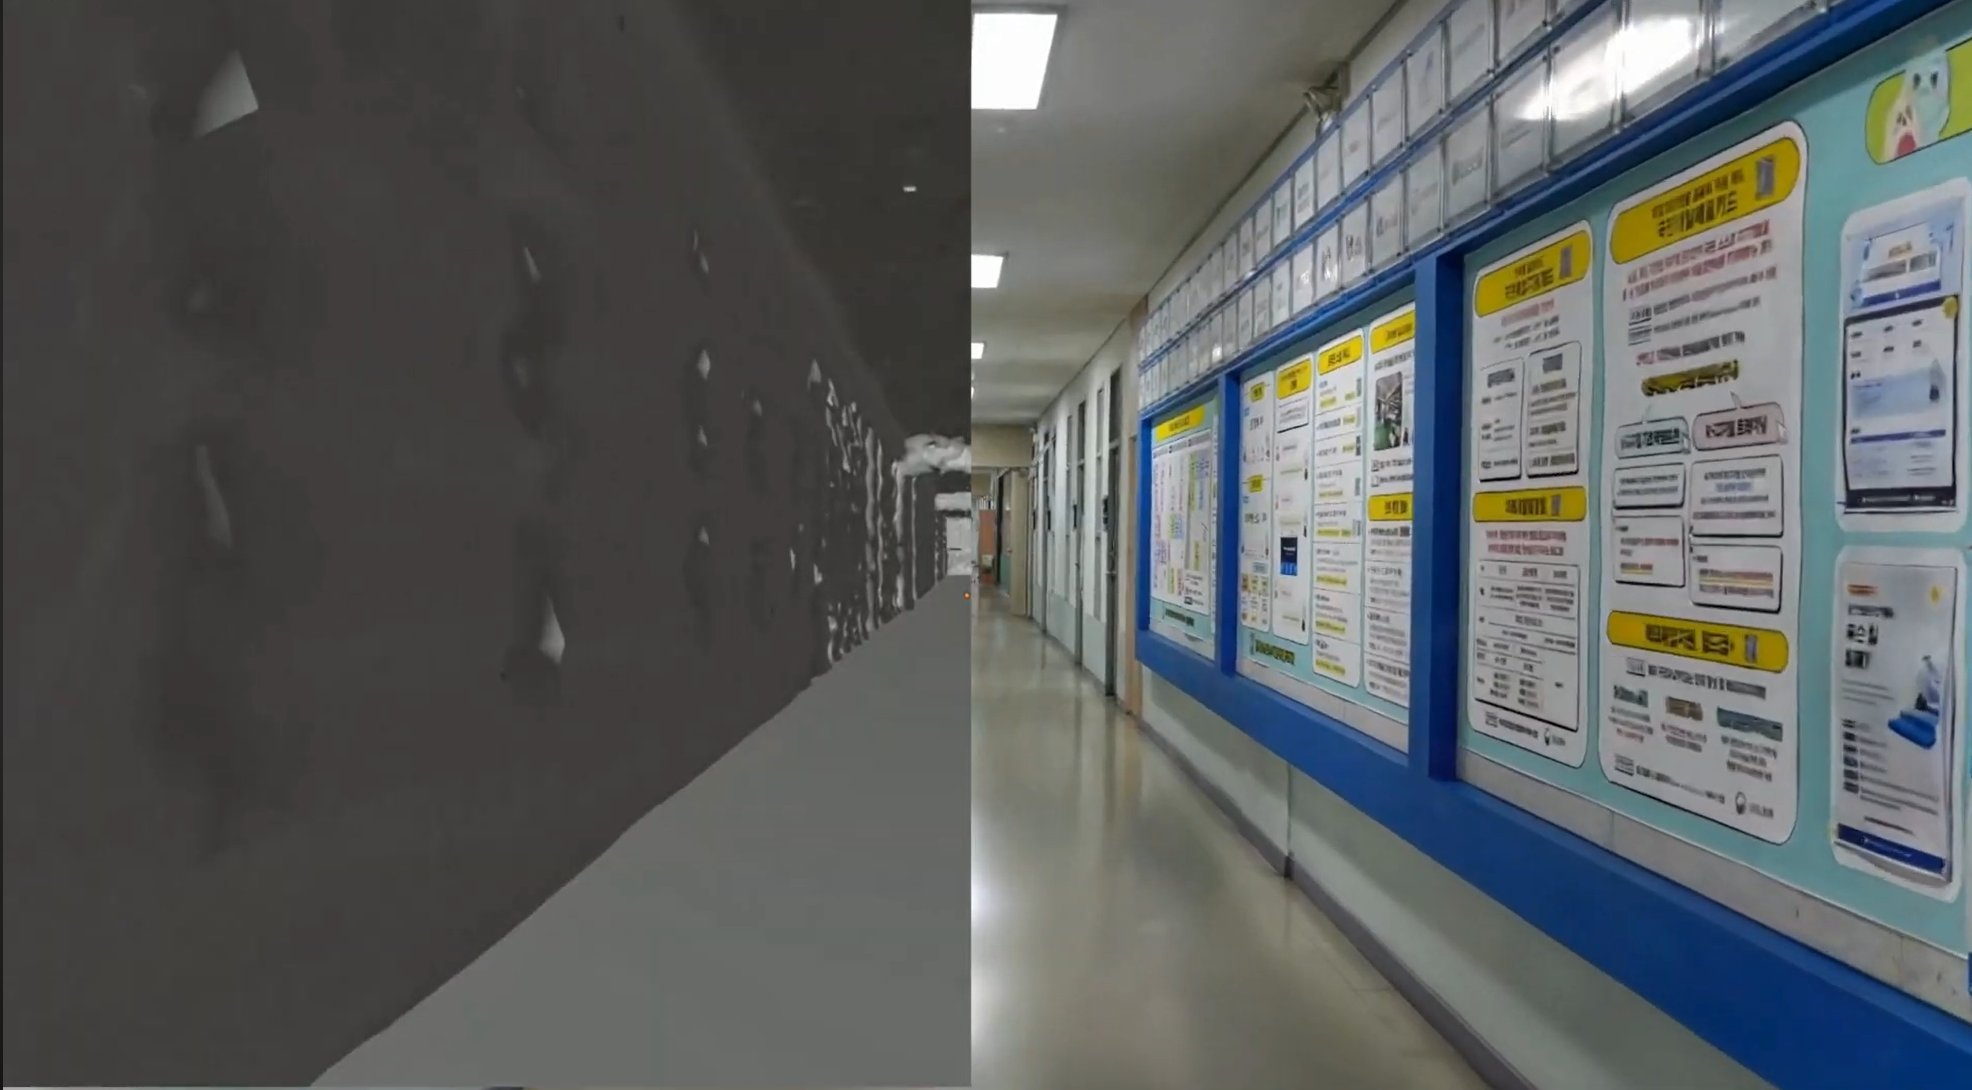
\includegraphics[width=0.98\linewidth]{figures/fig_3dgs_mesh.jpg}
\vspace{1.5mm}
\caption{\label{fig_3dgs_mesh}Digital twin representation of the campus corridor. Left: Sparse volumetric collision mesh generated using fVDB. Right: 3DGS render.}
\vspace{-2mm}
\end{center}
\end{figure}

We import these assets into Isaac Sim, where the collision boundaries are computed using the \textit{fVDB} representation. A ROS 2 bridge publishes virtual RGB-D sensor streams, visualizes the robot state in RViz, and routes velocity commands. The virtual camera's field-of-view and resolution are configured to match the physical D435i camera to reduce the visual gap. The pre-trained locomotion policy is then deployed on the Go2 model to maintain stable gaits within the simulated corridor.

\section{Experimental Results}
\subsection{Experimental Setup and Evaluation Methodology}

The navigation system consists of an Intel RealSense D435i RGB-D sensor, RTAB-Map \cite{ref2}, and the ROS 2 Nav2 stack. The sensor is mounted to the front torso of the Go2, and the virtual camera in simulation replicates its color and depth profiles to ensure consistency. Unlike monocular frameworks (e.g., \mbox{VR-Robo} \cite{ref5}) that suffer from depth ambiguity, the active depth sensor provides direct geometric measurements for local costmaps.

RTAB-Map uses visual keypoints (e.g., GFTT/ORB) for odometry and loop-closure detection. The depth stream is projected to construct a 3D octomap and a 2D occupancy grid. For low-latency obstacle avoidance, raw depth frames are converted to a pseudo-2D laser scan via the \textit{depthimage\_to\_}\allowbreak\textit{laserscan} package. The Nav2 global planner plans paths on the occupancy grid, while the DWB local planner uses the local costmap to compute steering commands $\mathbf{v}_{cmd}$.

To resolve the coordinate transform (TF) tree discrepancy, a custom bridge maps the tree as \textit{map} $\rightarrow$ \textit{odom} $\rightarrow$ \textit{world} $\rightarrow$ \textit{base}, where RTAB-Map publishes the \textit{map} $\rightarrow$ \textit{odom} transform and Isaac Sim links odometry to the world frame. This enables standard ROS 2 navigation in simulation. The system is evaluated by analyzing mapping consistency in both simulated and physical environments and qualitatively inspecting obstacle-aware replanning in simulation under locomotion-induced camera oscillations.

\subsection{Results and Evaluation}
We validated the navigation stack in a simulated 3DGS corridor (80~m long, 2.5~m wide) before physical deployment.

In simulation, the locomotion policy receives proprioceptive and exteroceptive (height-scan) inputs. Ray-casting queries the collision mesh to provide local elevation profiles for foot placement. The closed-loop navigation system in simulation is illustrated in Fig.~\ref{fig_sim_nav2}. The local planner (DWB) in the Nav2 stack generates velocity commands based on the synchronized costmap and path planning displayed in RViz (Fig.~\ref{fig_sim_nav2}, right). These commands are then sent to the trained RL locomotion policy controlling the virtual robot in Isaac Sim (Fig.~\ref{fig_sim_nav2}, left), which simulates the physical walking dynamics and camera motion. Virtual obstacles are inserted in the corridor to qualitatively verify obstacle-aware replanning. As shown in the RViz visualization (Fig.~\ref{fig_sim_nav2}, right), the local planner recalculates paths around the inserted obstacles, and the simulated robot follows the replanned trajectory (Fig.~\ref{fig_sim_nav2}, left).

\begin{figure}[H]
\begin{center}
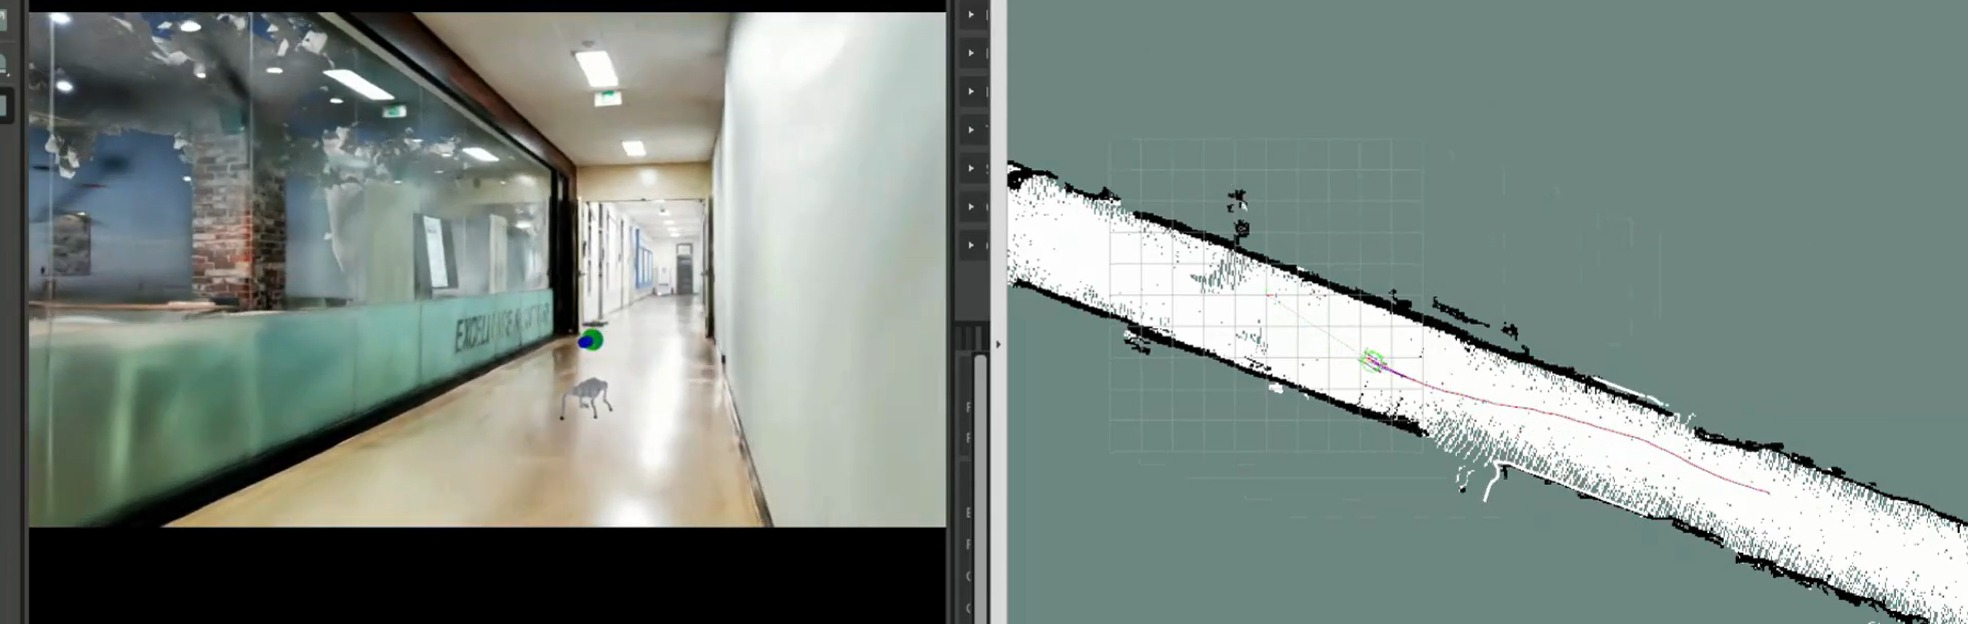
\includegraphics[width=0.98\linewidth]{figures/fig_sim_nav2.jpg}
\vspace{1.5mm}
\caption{\label{fig_sim_nav2}Autonomous navigation execution inside the reconstructed virtual environment, showing the simulated quadruped robot in Isaac Sim (left) and path planning/costmap synchronization in RViz (right).}
\end{center}
\end{figure}

The resulting mapping outputs generated during simulated navigation are shown in Fig.~\ref{fig_sim_validation}.

\begin{figure}[H]
\begin{center}
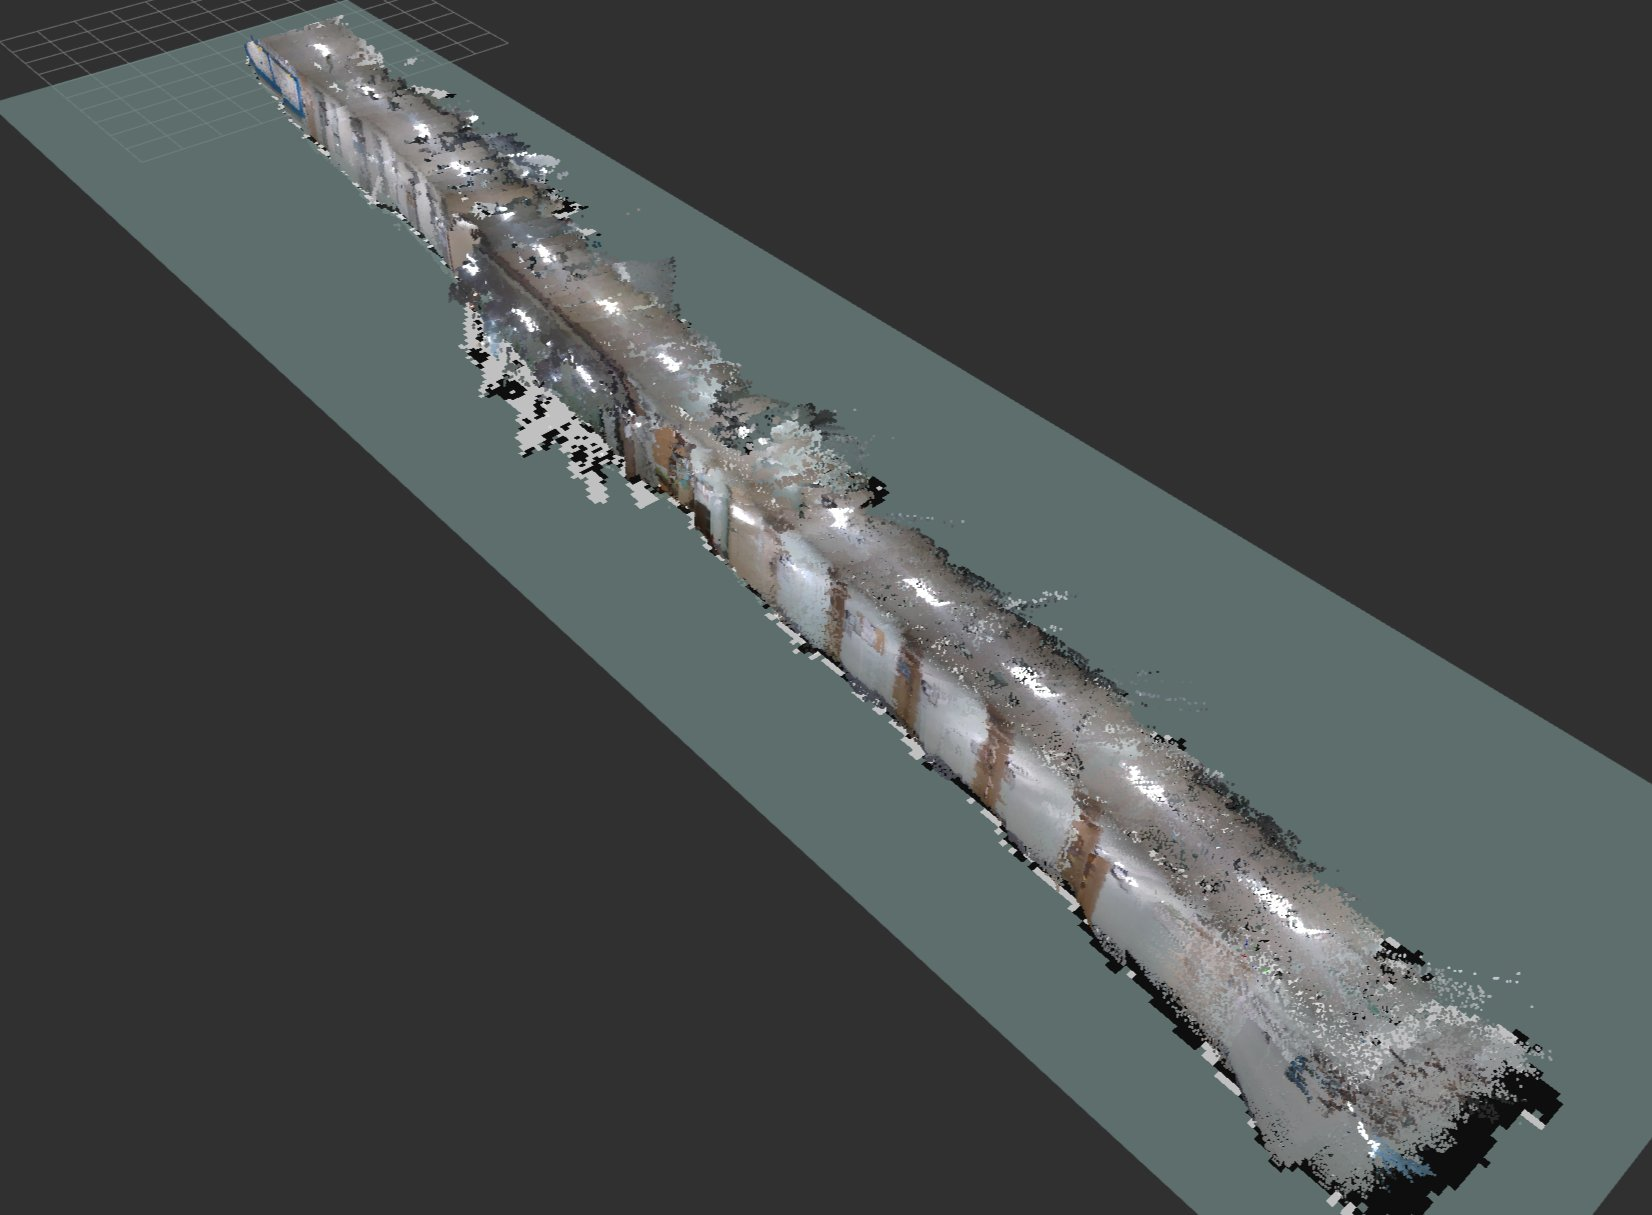
\includegraphics[width=0.83\linewidth, height=0.61\linewidth]{figures/fig_3d_map.jpg}
\hfill
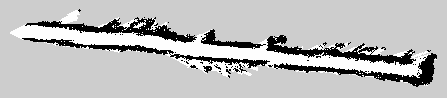
\includegraphics[width=0.134\linewidth, height=0.61\linewidth]{figures/fig_2d_map.png}
\vspace{1.5mm}
\caption{\label{fig_sim_validation}Visual mapping results in simulation. Left: Reconstructed 3D point cloud map from RTAB-Map. Right: Projected 2D occupancy grid map.}
\end{center}
\end{figure}

We deployed the proposed framework on a physical Unitree Go2 robot to navigate the campus corridor, as shown in Fig.~\ref{fig_real_deployment}. The robot is equipped with a front-facing Intel RealSense D435i camera and an NVIDIA Jetson Orin NX computer, running the entire navigation and mapping stack locally.

To reduce computational load on the Jetson Orin NX, the RL policy is bypassed, and commands are sent to the built-in Sport API via a ROS 2 bridge, reserving onboard resources for SLAM and path planning. The camera is connected via USB 3.0.

\begin{figure}[H]
\begin{center}
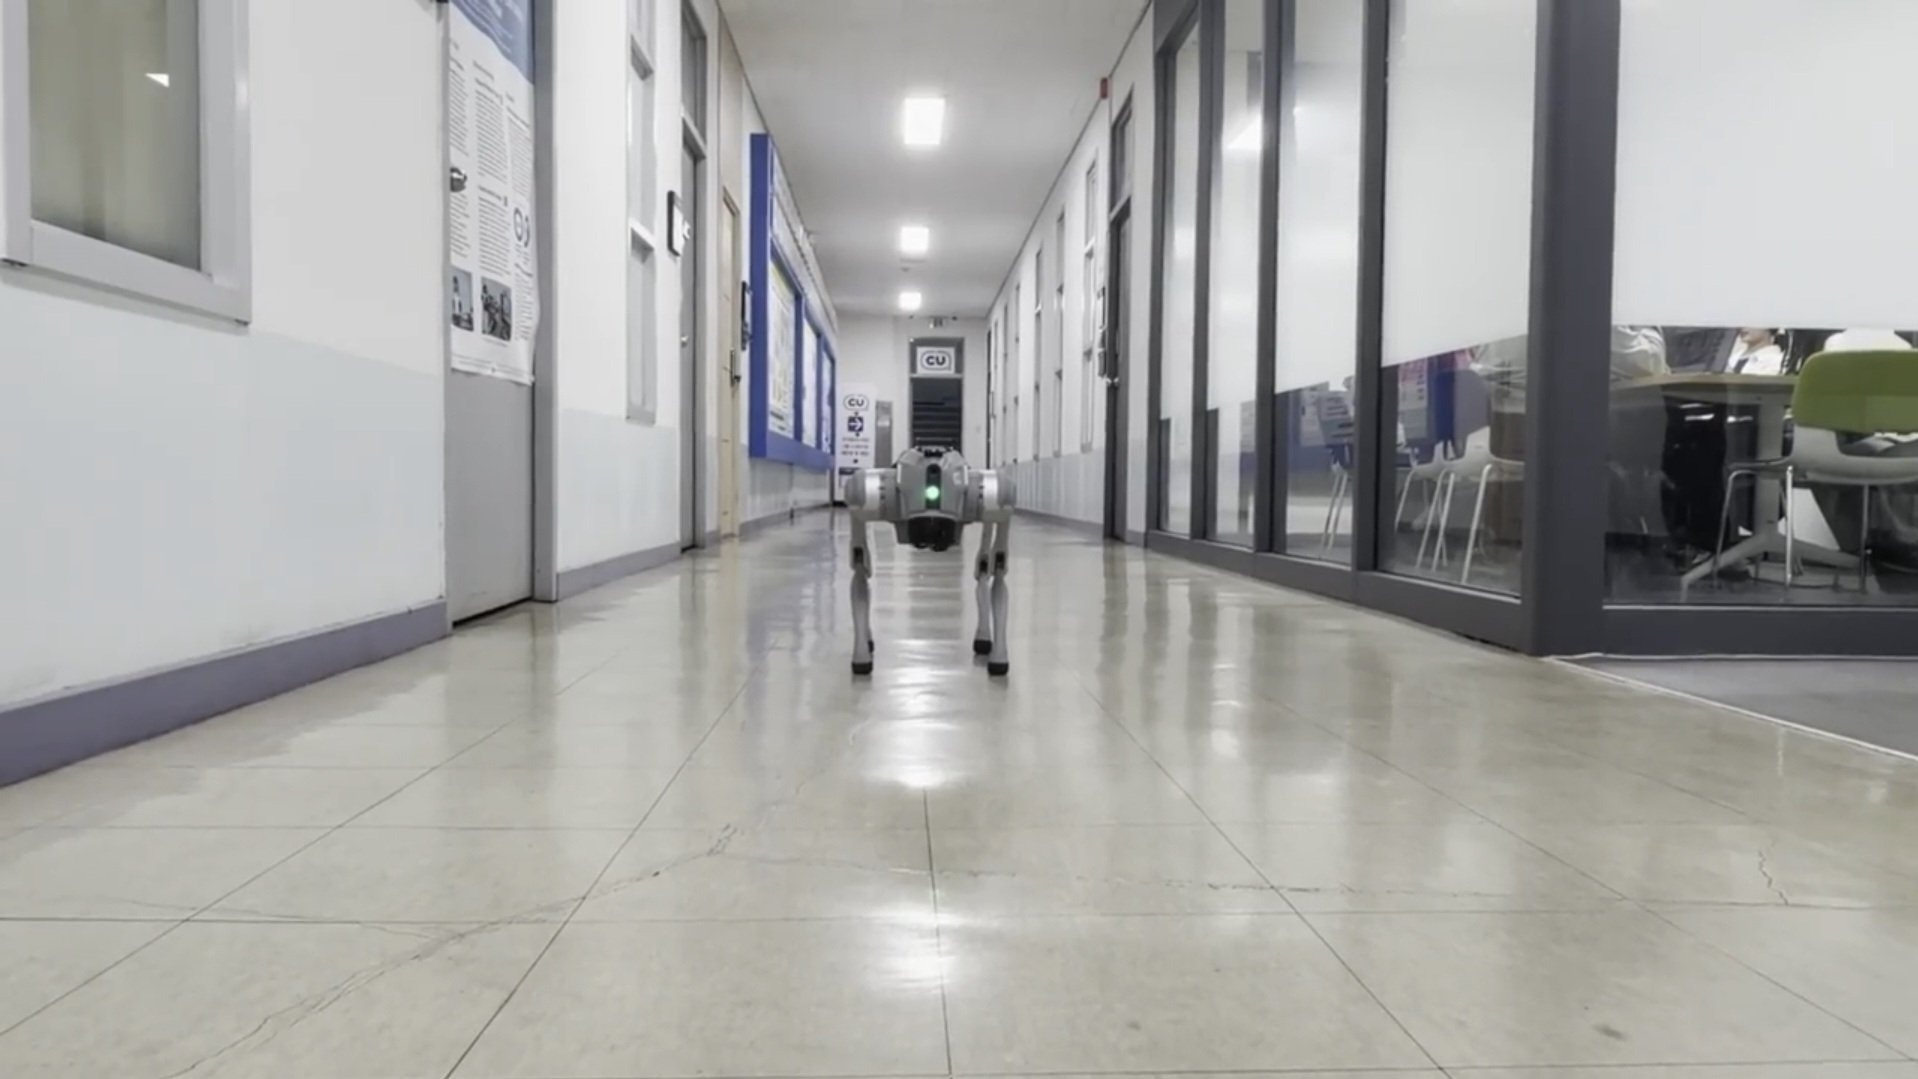
\includegraphics[width=0.98\linewidth]{figures/fig_real_robot.jpg}
\vspace{1.5mm}
\caption{\label{fig_real_deployment}Real-world experimental setup. The Unitree Go2 robot is equipped with an Intel RealSense D435i and Jetson Orin NX, running the entire navigation stack on-board.}
\end{center}
\end{figure}

Although the simulation used ROS 2 Jazzy (Ubuntu 24.04) and the physical robot used ROS 2 Foxy (Ubuntu 20.04), the same software architecture was maintained. This allowed parameters optimized under simulated camera noise to transfer directly to the physical platform without manual recalibration. RTAB-Map detected loop closures during walking, and the robot maintained a target velocity of $0.4$~m/s. These results indicate that the proposed pipeline enables practical transfer of navigation parameters to the physical robot.

\subsection{Limitations and Future Work}
Several limitations remain. First, physical deployment bypasses the learned locomotion policy and uses the built-in Sport API; thus, this work validates the transfer of navigation and mapping parameters rather than the learned controller itself. Second, the experiments are conducted in a mostly static corridor, and obstacle avoidance is evaluated qualitatively without repeated-trial success rates. Future work will include quantitative benchmarks for localization drift, map consistency, obstacle-avoidance success rate, dynamic obstacles, and edge optimization.

\section{Conclusion}
This paper presented a 3DGS-based sim-to-real validation pipeline for quadrupedal visual navigation. By combining a photorealistic digital twin with RL-generated walking dynamics, the framework enables RTAB-Map and Nav2 parameters to be tuned under visual and motion disturbances before deployment. Experiments on a Unitree Go2 show that the optimized navigation stack can be deployed through a ROS 2 bridge and the built-in Sport API without manual recalibration.

\section*{ACKNOWLEDGEMENT}
This research was supported by the National Research Foundation of Korea (NRF) grant funded by the Korean government (MSIT) (No. RS-2025-24683458).

\section*{USE OF AI TOOLS}
During the preparation of this work, the authors used Gemini (developed by Google) for grammar editing and style improvement of the manuscript. After using this tool, the authors reviewed and edited the content as needed and take full responsibility for the final text of the paper.
\begin{thebibliography}{99}

\bibitem{ref1}
J. Hwangbo, J. Lee, A. Dosovitskiy, D. Bellicoso, V. Tsounis, V. Koltun, and M. Hutter, ``Learning agile and dynamic motor skills for legged robots,'' \textit{Science Robotics}, vol. 4, no. 26, p. eaau5872, 2019.

\bibitem{ref2}
M. Labb{\'e} and F. Michaud, ``RTAB-Map as an open-source lidar and visual simultaneous localization and mapping library for large-scale and long-term online operation,'' arXiv preprint arXiv:2403.06341, 2024.

\bibitem{ref3}
S. Macenski, T. Foote, B. Gerkey, C. Lalancette, and W. Woodall, ``Robot Operating System 2: Design, architecture, and uses in the wild,'' \textit{Science Robotics}, vol. 7, no. 66, p. eabm6074, 2022.

\bibitem{ref4}
B. Kerbl, G. Kopanas, T. Leimk{\"u}hler, and G. Drettakis, ``3D Gaussian splatting for real-time radiance field rendering,'' \textit{ACM Transactions on Graphics}, vol. 42, no. 4, pp. 1--14, 2023.

\bibitem{ref5}
S. Zhu, L. Mou, D. Li, B. Ye, R. Huang, and H. Zhao, ``VR-Robo: A real-to-sim-to-real framework for visual robot navigation and locomotion,'' \textit{IEEE Robotics and Automation Letters}, vol. 10, no. 8, pp. 7875--7882, August 2025.

\bibitem{ref6}
J. Tan, T. Zhang, E. Coumans, A. Iscen, Y. Bai, D. Hafner, S. Bohez, and V. Vanhoucke, ``Sim-to-real: Learning agile locomotion for quadruped robots,'' in \textit{Proc. RSS}, 2018.

\bibitem{ref7}
N. Rudin, D. Hoeller, P. Reist, and M. Hutter, ``Learning to walk in minutes using massively parallel deep reinforcement learning,'' in \textit{Proc. CoRL}, 2022.

\bibitem{ref8}
R. Mur-Artal and J. D. Tard{\'o}s, ``ORB-SLAM2: An open-source SLAM system for monocular, stereo, and RGB-D cameras,'' \textit{IEEE Trans. Robotics}, vol. 33, no. 5, pp. 1255--1262, 2017.

\bibitem{ref9}
J. L. Sch{\"o}nberger and J.-M. Frahm, ``Structure-from-motion revisited,'' in \textit{Proc. CVPR}, pp. 4104--4113, 2016.

\bibitem{ref10}
N. Keetha, J. Karhade, K. M. Jatavallabhula, G. Yang, S. Scherer, D. Ramanan, and J. Luiten, ``SplaTAM: Splat, track \& map 3D Gaussians for dense RGB-D SLAM,'' in \textit{Proc. CVPR}, 2024.

\end{thebibliography}

\end{document}
